\documentclass{standalone}
\usepackage{tikz}
\usetikzlibrary{patterns, positioning}

\begin{document}
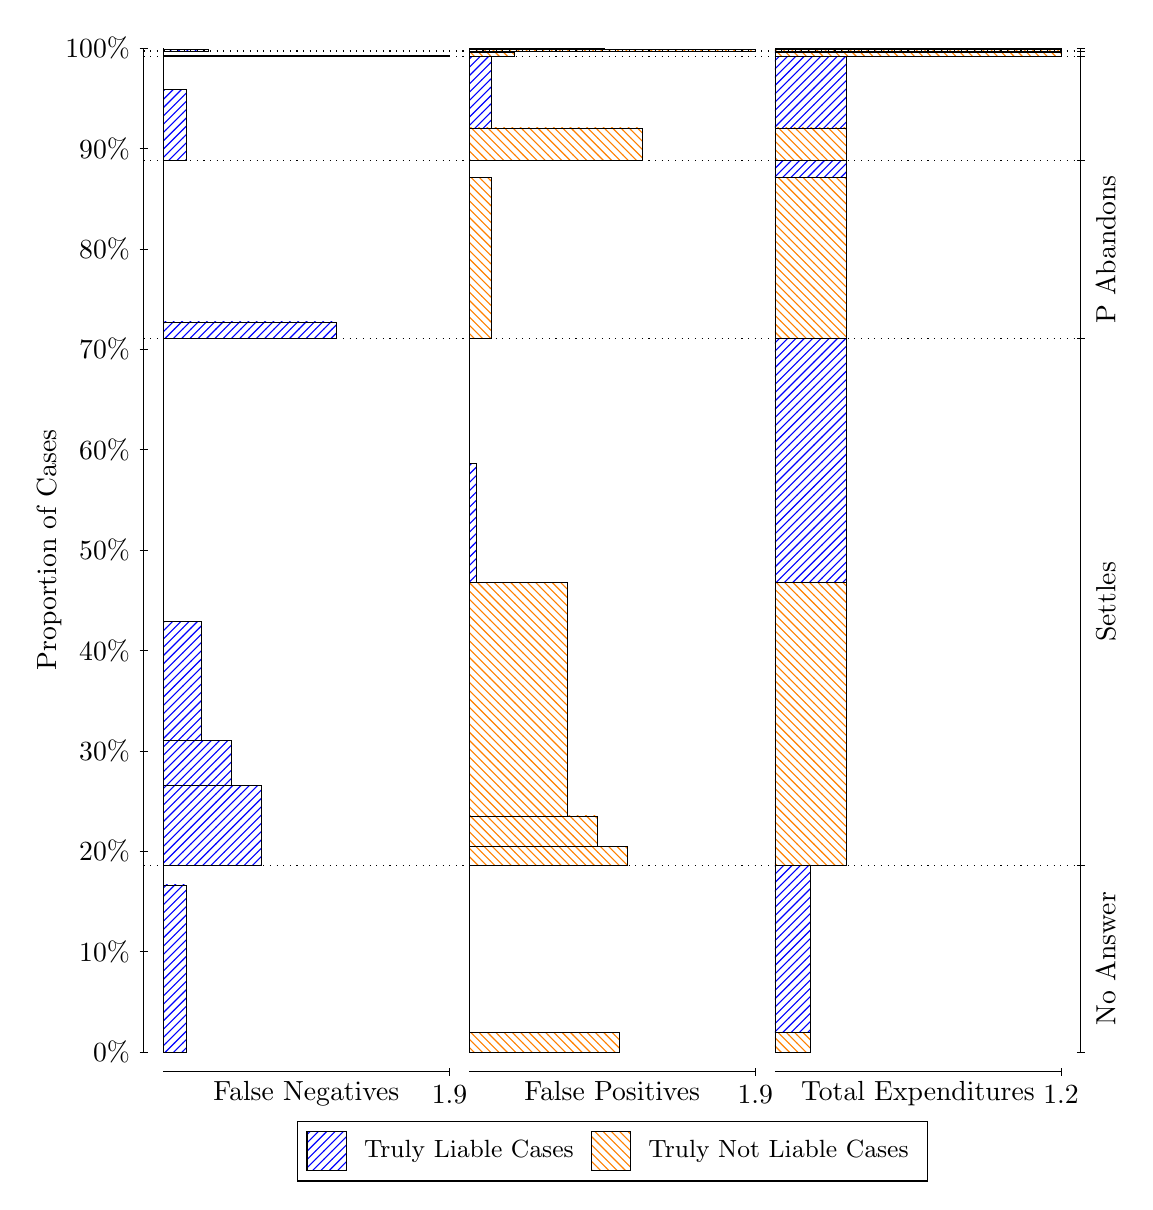
\begin{tikzpicture}
\draw[black, very thin] (1.5,1.75) -- (1.5,14.5);
\node[rotate=90, anchor=center] at (0.3, 8.125) {Proportion of Cases};
\draw[black, very thin] (1.45,1.75) -- (1.55,1.75);
\node[anchor=east] at (1.45, 1.75) {0\%};
\draw[black, very thin] (1.45,3.025) -- (1.55,3.025);
\node[anchor=east] at (1.45, 3.025) {10\%};
\draw[black, very thin] (1.45,4.3) -- (1.55,4.3);
\node[anchor=east] at (1.45, 4.3) {20\%};
\draw[black, very thin] (1.45,5.575) -- (1.55,5.575);
\node[anchor=east] at (1.45, 5.575) {30\%};
\draw[black, very thin] (1.45,6.85) -- (1.55,6.85);
\node[anchor=east] at (1.45, 6.85) {40\%};
\draw[black, very thin] (1.45,8.125) -- (1.55,8.125);
\node[anchor=east] at (1.45, 8.125) {50\%};
\draw[black, very thin] (1.45,9.4) -- (1.55,9.4);
\node[anchor=east] at (1.45, 9.4) {60\%};
\draw[black, very thin] (1.45,10.675) -- (1.55,10.675);
\node[anchor=east] at (1.45, 10.675) {70\%};
\draw[black, very thin] (1.45,11.95) -- (1.55,11.95);
\node[anchor=east] at (1.45, 11.95) {80\%};
\draw[black, very thin] (1.45,13.225) -- (1.55,13.225);
\node[anchor=east] at (1.45, 13.225) {90\%};
\draw[black, very thin] (1.45,14.5) -- (1.55,14.5);
\node[anchor=east] at (1.45, 14.5) {100\%};

\draw[black, very thin] (13.4,1.75) -- (13.4,14.5);
\draw[black, very thin] (13.35,1.75) -- (13.45,1.75);
\node[anchor=west] at (13.35, 1.75) {};
\draw[black, very thin] (13.35,4.1222) -- (13.45,4.1222);
\node[anchor=west] at (13.35, 4.1222) {};
\draw[black, very thin] (13.35,10.81) -- (13.45,10.81);
\node[anchor=west] at (13.35, 10.81) {};
\draw[black, very thin] (13.35,13.072) -- (13.45,13.072);
\node[anchor=west] at (13.35, 13.072) {};
\draw[black, very thin] (13.35,14.389) -- (13.45,14.389);
\node[anchor=west] at (13.35, 14.389) {};
\draw[black, very thin] (13.35,14.462) -- (13.45,14.462);
\node[anchor=west] at (13.35, 14.462) {};
\draw[black, very thin] (13.35,14.5) -- (13.45,14.5);
\node[anchor=west] at (13.35, 14.5) {};

\draw[black, very thin, pattern color=blue, pattern=north east lines] (1.75,1.75) rectangle (2.0368,3.8726);
\draw[black, very thin, pattern color=orange, pattern=north west lines] (1.75,3.8726) rectangle (1.75,4.1222);
\draw[black, very thin, pattern color=blue, pattern=north east lines] (1.75,4.1222) rectangle (2.993,5.1374);
\draw[black, very thin, pattern color=blue, pattern=north east lines] (1.75,5.1374) rectangle (2.6105,5.711);
\draw[black, very thin, pattern color=blue, pattern=north east lines] (1.75,5.711) rectangle (2.2281,7.2205);
\draw[black, very thin, pattern color=orange, pattern=north west lines] (1.75,7.2205) rectangle (1.75,10.81);
\draw[black, very thin, pattern color=blue, pattern=north east lines] (1.75,10.81) rectangle (3.9491,11.022);
\draw[black, very thin, pattern color=orange, pattern=north west lines] (1.75,11.022) rectangle (1.75,13.072);
\draw[black, very thin, pattern color=blue, pattern=north east lines] (1.75,13.072) rectangle (2.0368,13.977);
\draw[black, very thin, pattern color=orange, pattern=north west lines] (1.75,13.977) rectangle (1.75,14.389);
\draw[black, very thin, pattern color=blue, pattern=north east lines] (1.75,14.389) rectangle (5.3833,14.408);
\draw[black, very thin, pattern color=orange, pattern=north west lines] (1.75,14.408) rectangle (1.75,14.462);
\draw[black, very thin, pattern color=blue, pattern=north east lines] (1.75,14.462) rectangle (2.3237,14.482);
\draw[black, very thin, pattern color=orange, pattern=north west lines] (1.75,14.482) rectangle (1.75,14.5);
\draw[black, very thin, pattern color=orange, pattern=north west lines] (5.6333,1.75) rectangle (7.5456,1.9996);
\draw[black, very thin, pattern color=blue, pattern=north east lines] (5.6333,1.9996) rectangle (5.6333,4.1222);
\draw[black, very thin, pattern color=orange, pattern=north west lines] (5.6333,4.1222) rectangle (7.6412,4.3611);
\draw[black, very thin, pattern color=orange, pattern=north west lines] (5.6333,4.3611) rectangle (7.2588,4.7471);
\draw[black, very thin, pattern color=orange, pattern=north west lines] (5.6333,4.7471) rectangle (6.8763,7.7121);
\draw[black, very thin, pattern color=blue, pattern=north east lines] (5.6333,7.7121) rectangle (5.7289,9.2215);
\draw[black, very thin, pattern color=blue, pattern=north east lines] (5.6333,9.2215) rectangle (5.6333,10.81);
\draw[black, very thin, pattern color=orange, pattern=north west lines] (5.6333,10.81) rectangle (5.9202,12.86);
\draw[black, very thin, pattern color=blue, pattern=north east lines] (5.6333,12.86) rectangle (5.6333,13.072);
\draw[black, very thin, pattern color=orange, pattern=north west lines] (5.6333,13.072) rectangle (7.8325,13.485);
\draw[black, very thin, pattern color=blue, pattern=north east lines] (5.6333,13.485) rectangle (5.9202,14.389);
\draw[black, very thin, pattern color=orange, pattern=north west lines] (5.6333,14.389) rectangle (6.207,14.444);
\draw[black, very thin, pattern color=blue, pattern=north east lines] (5.6333,14.444) rectangle (5.6333,14.462);
\draw[black, very thin, pattern color=orange, pattern=north west lines] (5.6333,14.462) rectangle (9.2667,14.481);
\draw[black, very thin, pattern color=blue, pattern=north east lines] (5.6333,14.481) rectangle (7.3544,14.5);
\draw[black, very thin, pattern color=orange, pattern=north west lines] (9.5167,1.75) rectangle (9.9708,1.9996);
\draw[black, very thin, pattern color=blue, pattern=north east lines] (9.5167,1.9996) rectangle (9.9708,4.1222);
\draw[black, very thin, pattern color=orange, pattern=north west lines] (9.5167,4.1222) rectangle (10.425,7.7121);
\draw[black, very thin, pattern color=blue, pattern=north east lines] (9.5167,7.7121) rectangle (10.425,10.81);
\draw[black, very thin, pattern color=orange, pattern=north west lines] (9.5167,10.81) rectangle (10.425,12.86);
\draw[black, very thin, pattern color=blue, pattern=north east lines] (9.5167,12.86) rectangle (10.425,13.072);
\draw[black, very thin, pattern color=orange, pattern=north west lines] (9.5167,13.072) rectangle (10.425,13.485);
\draw[black, very thin, pattern color=blue, pattern=north east lines] (9.5167,13.485) rectangle (10.425,14.389);
\draw[black, very thin, pattern color=orange, pattern=north west lines] (9.5167,14.389) rectangle (13.15,14.444);
\draw[black, very thin, pattern color=blue, pattern=north east lines] (9.5167,14.444) rectangle (13.15,14.462);
\draw[black, very thin, pattern color=orange, pattern=north west lines] (9.5167,14.462) rectangle (13.15,14.481);
\draw[black, very thin, pattern color=blue, pattern=north east lines] (9.5167,14.481) rectangle (13.15,14.5);
\draw[black, dotted] (1.5,4.1222) -- (13.4,4.1222);
\draw[black, dotted] (1.5,10.81) -- (13.4,10.81);
\draw[black, dotted] (1.5,13.072) -- (13.4,13.072);
\draw[black, dotted] (1.5,14.389) -- (13.4,14.389);
\draw[black, dotted] (1.5,14.462) -- (13.4,14.462);
\draw[black, very thin] (1.75,1.5) -- (5.3833,1.5);
\node[anchor=north] at (3.5667, 1.5) {False Negatives};
\draw[black, very thin] (5.3833,1.45) -- (5.3833,1.55);
\node[anchor=north] at (5.3833, 1.45) {1.9};

\draw[black, very thin] (5.6333,1.5) -- (9.2667,1.5);
\node[anchor=north] at (7.45, 1.5) {False Positives};
\draw[black, very thin] (9.2667,1.45) -- (9.2667,1.55);
\node[anchor=north] at (9.2667, 1.45) {1.9};

\draw[black, very thin] (9.5167,1.5) -- (13.15,1.5);
\node[anchor=north] at (11.333, 1.5) {Total Expenditures};
\draw[black, very thin] (13.15,1.45) -- (13.15,1.55);
\node[anchor=north] at (13.15, 1.45) {1.2};

\node[black, centered, rotate=90] at (13.72, 2.9361) {No Answer};
\node[black, centered, rotate=90] at (13.72, 7.4663) {Settles};
\node[black, centered, rotate=90] at (13.72, 11.941) {P Abandons};




\draw (7.449999999999999,1.5) node[draw=none] (baseCoordinate) {};
\begin{scope}[align=center]
        \matrix[scale=0.5, draw=black, below=0.5cm of baseCoordinate, nodes={draw}, column sep=0.1cm]{
            \node[rectangle, draw, minimum width=0.5cm, minimum height=0.5cm, pattern=north east lines, pattern color=blue] {}; &
            \node[draw=none, font=\small] (B) {Truly Liable Cases}; &
            \node[rectangle, draw, minimum width=0.5cm, minimum height=0.5cm, pattern=north west lines, pattern color=orange] {}; &
            \node[draw=none, font=\small] (B) {Truly Not Liable Cases}; \\
            };
\end{scope}

\end{tikzpicture}
\end{document}